% Apresentação da PoC OCR-06 no IV Workshop Acadêmico do Registro Civil (INE5448), 15 min + 5 min.
% Segue a estrutura e a paleta do template da disciplina: contexto, problema e projeto primeiro,
% resultados no final. Figuras geradas por ocr06/scripts/figs_workshop.py.
\documentclass[aspectratio=169,t,11pt]{beamer}

\usepackage[utf8]{inputenc}
\usepackage[T1]{fontenc}
\usepackage[brazilian]{babel}
\usepackage[semibold]{sourceserifpro}
\usepackage[default,semibold]{sourcesanspro}
\usepackage[scale=0.88]{sourcecodepro}
\usepackage{booktabs}
\usepackage{array}
\usepackage{pifont}
\usepackage{tikz}
\usetikzlibrary{positioning,arrows.meta,fit,backgrounds,calc}
\usepackage{qrcode}
\graphicspath{{figs/}}

\usetheme{default}
\usefonttheme{professionalfonts}
\setbeamertemplate{navigation symbols}{}
\setbeamersize{text margin left=8mm, text margin right=8mm}
\setbeamertemplate{itemize items}[circle]
\setbeamercolor{itemize item}{fg=gold}
\setbeamercolor{itemize subitem}{fg=gold}

% ---- Paleta do template ----------------------------------------------
\definecolor{deepteal}{RGB}{18,50,46}
\definecolor{gold}{RGB}{199,154,107}
\definecolor{labelclr}{RGB}{176,84,62}
\definecolor{rulegray}{RGB}{205,205,200}
\definecolor{tinta}{RGB}{70,72,70}
\definecolor{bom}{HTML}{1B8A62}
\definecolor{ruim}{HTML}{C0392B}
\setbeamercolor{normal text}{fg=black!88,bg=white}
\setbeamercolor{background canvas}{bg=white}

% ---- Macros de layout do template ------------------------------------
\newcommand{\footlogo}{
\includegraphics[height=6mm,keepaspectratio]{logo_labrec_onrcpn.png}}
\newcommand{\hrulec}[2]{\par\nointerlineskip{\color{#1}\hrule height #2}\nointerlineskip\par}
\newcommand{\framenumtwo}{\ifnum\insertframenumber<10 0\fi\insertframenumber}
\newcommand{\slidehead}[1]{%
  {\ttfamily\scriptsize\textcolor{labelclr}{\framenumtwo}\hspace{1.4em}%
   \textcolor{black!62}{\MakeUppercase{#1}}}\par\vspace{0.6mm}%
  \hrulec{rulegray}{0.4pt}\vspace{2.6mm}}
\newcommand{\slidetitle}[1]{{\rmfamily\fontsize{21}{25}\selectfont\color{deepteal}#1\par}}
\newcommand{\slidesub}[1]{\vspace{0.7mm}{\small\color{tinta}#1\par}}
\newcommand{\slidesubserif}[1]{\vspace{1.2mm}{\rmfamily\itshape\fontsize{13.5}{17}\selectfont\color{gold!85!black}#1\par}}
\newcommand{\lbl}[1]{{\ttfamily\fontsize{7.6}{9.5}\selectfont\textcolor{labelclr}{\MakeUppercase{#1}}}\par\vspace{1mm}}
\newcommand{\coltop}{\hrulec{deepteal}{0.9pt}\vspace{1.5mm}}
\newcommand{\thinrule}{\par\vspace{1.1mm}\hrulec{rulegray}{0.4pt}\vspace{1.1mm}}
\newcommand{\sidenote}[1]{%
  \noindent{\color{gold}\rule[-1.2mm]{1.2pt}{4.6mm}}\hspace{2mm}%
  {\rmfamily\itshape\small #1}\par}
\newcommand{\darkband}[1]{%
  \begin{tikzpicture}
    \node[fill=deepteal,minimum width=\linewidth,minimum height=12mm,
          inner sep=3.5mm,align=left,text width=\linewidth-7mm,text=white]
         {\rmfamily\fontsize{14.5}{18}\selectfont #1};
  \end{tikzpicture}}
\setbeamertemplate{footline}{%
  \hbox to\paperwidth{\hspace{8mm}%
    \raisebox{1.5mm}{\ttfamily\scriptsize\color{black!45}\insertframenumber}%
    \hfill\footlogo\hspace{8mm}}\vspace{1.2mm}}
\newenvironment{darkframe}{%
  \begingroup
  \setbeamercolor{background canvas}{bg=deepteal}
  \setbeamertemplate{footline}{}%
}{\endgroup}

\newcommand{\erro}[1]{\textcolor{ruim}{\textbf{#1}}}
\newcommand{\marcacerto}{\textcolor{bom}{\ding{51}}}
\newcommand{\marcaerro}{\textcolor{ruim}{\ding{55}}}
\newcommand{\leitura}[3]{{\footnotesize\renewcommand{\arraystretch}{1.08}\begin{tabular}{@{}l@{\hspace{0.8em}}l@{}}\textcolor{tinta}{Gabarito} & #1 \\ \textcolor{tinta}{Chandra OCR 2} & #2 \\ \textcolor{tinta}{lora\_v2} & #3 \\\end{tabular}}}
% a mesma certidão com os campos certos e errados, e o placar ao lado
\newcommand{\demonstracao}[4]{%
  \begin{frame}[plain]
  \begin{tikzpicture}[remember picture,overlay]
    \node[anchor=west,inner sep=0] at (current page.west) {\includegraphics[height=\paperheight]{#1}};
    \node[anchor=center,align=flush center,text width=4.1cm] at ($(current page.east)+(-2.37cm,0)$) {
      {\ttfamily\fontsize{7.6}{10}\selectfont\textcolor{labelclr}{DEMONSTRAÇÃO}\par}
      \vspace{1.5mm}
      {\rmfamily\fontsize{15.5}{19}\selectfont\color{deepteal}#2\par}
      \vspace{2mm}
      {\rmfamily\fontsize{52}{56}\selectfont\color{deepteal}#3\par}
      {\normalsize de 21 campos certos\par}
      \vspace{3mm}
      {\small\color{tinta}#4\par}
    };
  \end{tikzpicture}
  \end{frame}}

\begin{document}

% =====================================================================
% CAPA
% =====================================================================
\begin{darkframe}
\begin{frame}[plain]
\color{white}
\vspace{5mm}
\begin{columns}[T,onlytextwidth]
\begin{column}{0.66\textwidth}
  {\ttfamily\scriptsize\color{gold}APRESENTAÇÃO}\hspace{2mm}%
  {\color{white!40!deepteal}\rule[1mm]{0.62\linewidth}{0.4pt}}\par
  \vspace{7mm}
  {\rmfamily\fontsize{27}{32}\selectfont OCR Adaptativo com Aprendizagem Assistida\par}
  \vspace{3mm}
  {\fontsize{12.5}{16}\selectfont Ajuste fino do Chandra OCR 2 para campos manuscritos de certidões de Registro Civil\par}
  \vspace{5mm}
  {\rmfamily\itshape\fontsize{13}{16}\selectfont\color{gold}Gabriel Salmoria\par}
  \vspace{7mm}
  \hrulec{white!35!deepteal}{0.4pt}\vspace{2.5mm}
  \begin{columns}[T,onlytextwidth]
    \begin{column}{0.5\textwidth}
      {\ttfamily\fontsize{6.8}{8}\selectfont\color{white!70!deepteal}TUTOR}\par\vspace{1mm}
      {\small Lucas Mayr}
    \end{column}
    \begin{column}{0.5\textwidth}
      {\ttfamily\fontsize{6.8}{8}\selectfont\color{white!70!deepteal}DATA}\par\vspace{1mm}
      {\small 23 de novembro de 2026}
    \end{column}
  \end{columns}
\end{column}
\begin{column}{0.30\textwidth}
  \centering
  \vspace{5mm}
  
\includegraphics[width=38mm,keepaspectratio]{workshop-logo.png}
\end{column}
\end{columns}
\end{frame}
\end{darkframe}

% =====================================================================
% ROTEIRO
% =====================================================================
\begin{frame}
\slidehead{Roteiro}
\slidetitle{Estrutura da apresentação}
\vspace{7mm}
\begin{columns}[t,onlytextwidth]
\begin{column}{0.30\textwidth}\coltop \lbl{01} {\rmfamily\Large Contexto e problema}\end{column}
\begin{column}{0.30\textwidth}\coltop \lbl{02} {\rmfamily\Large Solução e arquitetura}\end{column}
\begin{column}{0.30\textwidth}\coltop \lbl{03} {\rmfamily\Large Dados e segurança}\end{column}
\end{columns}
\vspace{8mm}
\begin{columns}[t,onlytextwidth]
\begin{column}{0.30\textwidth}\coltop \lbl{04} {\rmfamily\Large Metodologia e avaliação}\end{column}
\begin{column}{0.30\textwidth}\coltop \lbl{05} {\rmfamily\Large Resultados e limites}\end{column}
\begin{column}{0.30\textwidth}\coltop \lbl{06} {\rmfamily\Large Próximos passos}\end{column}
\end{columns}
\end{frame}

% =====================================================================
% CONTEXTO
% =====================================================================
\begin{frame}
\slidehead{Contexto}
\slidetitle{Contexto e motivação}
\vspace{4mm}
\hrulec{rulegray}{0.4pt}\vspace{3.5mm}
\begin{columns}[T,onlytextwidth]
  \begin{column}{0.22\textwidth}\lbl{cenário}\end{column}
  \begin{column}{0.76\textwidth}Em 2023 foram registrados 2,5 milhões de nascimentos, 1,4 milhão de óbitos e 941 mil casamentos (IBGE), e cada certidão traz vários nomes de pessoas.\end{column}
\end{columns}
\vspace{3.5mm}\hrulec{rulegray}{0.4pt}\vspace{3.5mm}
\begin{columns}[T,onlytextwidth]
  \begin{column}{0.22\textwidth}\lbl{público envolvido}\end{column}
  \begin{column}{0.76\textwidth}Oficiais e escreventes, que transcrevem e conferem os registros, e os cidadãos com nomes pouco comuns.\end{column}
\end{columns}
\vspace{3.5mm}\hrulec{rulegray}{0.4pt}\vspace{3.5mm}
\begin{columns}[T,onlytextwidth]
  \begin{column}{0.22\textwidth}\lbl{motivação}\end{column}
  \begin{column}{0.76\textwidth}OCRs baseados em modelos de linguagem visual (VLMs) já leem manuscrito, mas cada nome lido errado volta para correção manual, e o modelo repete o erro no documento seguinte.\end{column}
\end{columns}
\vspace{3.5mm}\hrulec{rulegray}{0.4pt}
\end{frame}

% =====================================================================
% PROBLEMA
% =====================================================================
\begin{frame}
\slidehead{Problema}
\slidetitle{Nomes raros viram nomes comuns}
\vspace{2.5mm}
\darkband{O OCR troca o nome raro pelo mais provável, e ajustá-lo com certidões reais exporia dados pessoais.}
\vspace{1.5mm}
\begin{columns}[T,onlytextwidth]
\begin{column}{0.53\textwidth}
  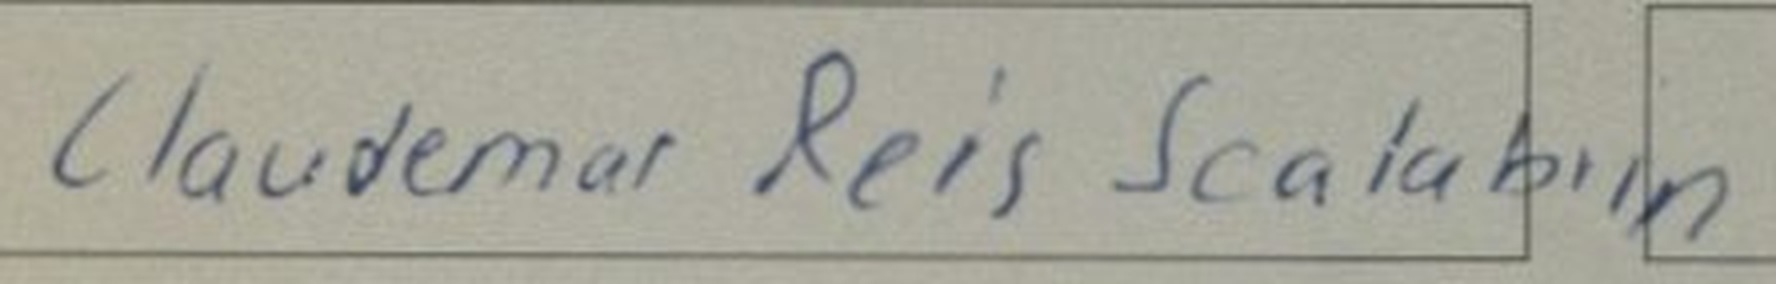
\includegraphics[width=\linewidth]{ex_claudemar.jpg}\par
  \vspace{2mm}
  {\normalsize
  \begin{tabular}{@{}l@{\hspace{1em}}l@{}}
  \textcolor{tinta}{Escrito} & Claudemar Reis Scalabrin \\
  \textcolor{tinta}{Chandra OCR 2} & Claude\erro{mi}r Reis Scalabrin \\
  \end{tabular}\par}
\end{column}
\begin{column}{0.43\textwidth}
  \small
  \lbl{impacto} Uma letra errada já é um erro no registro \thinrule
  \lbl{limitação atual} Nos testes, o Chandra lê sem erro 56\% dos campos \thinrule
  \lbl{oportunidade} Treinar com nomes públicos e certidões sintéticas
\end{column}
\end{columns}
\end{frame}

% =====================================================================
% OBJETIVOS
% =====================================================================
\begin{frame}
\slidehead{Objetivos}
\slidetitle{Objetivos do projeto}
\vspace{5mm}
\begin{columns}[T,onlytextwidth]
\begin{column}{0.44\textwidth}
  \lbl{objetivo geral}
  {\rmfamily\fontsize{16.5}{21}\selectfont Melhorar a leitura dos campos manuscritos de certidões, principalmente nomes nunca vistos, sem treinar com dados de pessoas reais\par}
\end{column}
\begin{column}{0.50\textwidth}
  \lbl{objetivos específicos}
  \hrulec{rulegray}{0.4pt}\vspace{2.5mm}
  \textbf{01}\quad Gerar dados sintéticos com nomes amostrados de estatísticas públicas
  \vspace{2.5mm}\hrulec{rulegray}{0.4pt}\vspace{2.5mm}
  \textbf{02}\quad Ajustar o Chandra OCR 2 com LoRA e medir o ganho em nomes fora do treino
  \vspace{2.5mm}\hrulec{rulegray}{0.4pt}\vspace{2.5mm}
  \textbf{03}\quad Quantizar o modelo e medir o custo em acurácia, memória e tempo
  \vspace{2.5mm}\hrulec{rulegray}{0.4pt}
\end{column}
\end{columns}
\end{frame}

% =====================================================================
% SOLUÇÃO
% =====================================================================
\begin{frame}
\slidehead{Solução}
\slidetitle{Solução proposta}
\slidesubserif{Ajuste fino com LoRA do Chandra OCR 2, só com certidões sintéticas}
\vspace{6mm}
\begin{columns}[t,onlytextwidth]
\begin{column}{0.29\textwidth}\coltop \lbl{entrada}
  Imagem da página inteira da certidão, com lado maior de 2.048 px\end{column}
\begin{column}{0.03\textwidth}\vspace{9mm}\centering\textcolor{gold}{$\rightarrow$}\end{column}
\begin{column}{0.29\textwidth}\coltop \lbl{processamento}
  Chandra OCR 2 (derivado do Qwen3.5-4B) com adaptador LoRA de 130 MB, servido pelo vLLM\end{column}
\begin{column}{0.03\textwidth}\vspace{9mm}\centering\textcolor{gold}{$\rightarrow$}\end{column}
\begin{column}{0.29\textwidth}\coltop \lbl{saída}
  HTML com o texto e a posição de cada bloco, para conferir cada campo sobre a imagem\end{column}
\end{columns}
\vfill
\lbl{saída real do modelo para um campo}
{\ttfamily\fontsize{7.7}{10}\selectfont <div data-bbox=\textquotedbl 98 552 377 577\textquotedbl{} data-label=\textquotedbl Text\textquotedbl><p><i>\textcolor{labelclr}{Claudemar Reis Scalabrin}</i></p></div>\par}
\vspace{2mm}
\end{frame}

% =====================================================================
% ARQUITETURA
% =====================================================================
\begin{frame}
\slidehead{Arquitetura}
\slidetitle{Arquitetura da solução}
\vspace{4.5mm}
\centering
\begin{tikzpicture}[
    font=\fontsize{8.6}{10.4}\selectfont,
    box/.style={draw=deepteal, line width=0.5pt, rounded corners=2pt, align=flush center, minimum height=1.02cm, text width=2.18cm, fill=white},
    forte/.style={box, fill=gold!22},
    arr/.style={-{Stealth[length=1.8mm]}, draw=deepteal, line width=0.6pt},
    lane/.style={draw=rulegray, fill=black!2, rounded corners=3pt, inner sep=5pt}]
  \node[box] (fontes) {IBGE, TSE\\e Receita};
  \node[box, right=0.5cm of fontes] (lexico) {Léxico e partição de nomes};
  \node[forte, right=0.5cm of lexico] (gerador) {Gerador de certidões};
  \node[box, right=0.5cm of gerador] (alvos) {Gabaritos no HTML nativo};
  \node[box, right=0.5cm of alvos] (conj) {Treino: 3.500\\ Teste: 294};
  \node[box, below=0.28cm of gerador] (ocrsd) {OCRSD\\(T. Siqueira)};
  \draw[arr] (fontes) -- (lexico);
  \draw[arr] (lexico) -- (gerador);
  \draw[arr] (gerador) -- (alvos);
  \draw[arr] (alvos) -- (conj);
  \draw[arr] (ocrsd) -- node[right, font=\fontsize{7}{8}\selectfont, text=tinta] {modelos} (gerador);
  \draw[arr] (ocrsd.east) -| node[pos=0.25, below, font=\fontsize{7}{8}\selectfont, text=tinta] {1.000 páginas} (conj.south);
  \begin{scope}[on background layer]
    \node[lane, fit=(fontes)(conj)(ocrsd), label={[font=\ttfamily\fontsize{7.4}{8}\selectfont, text=labelclr, anchor=south west, inner sep=1.5pt]north west:DADOS (CPU)}] (l1) {};
  \end{scope}
  \node[box, below=1.02cm of ocrsd.south -| fontes] (chandra) {Chandra OCR 2\\(BF16)};
  \node[forte, right=0.5cm of chandra] (lora) {Treino LoRA\\(peft)};
  \node[box, right=0.5cm of lora] (quant) {Fusão, FP8\\e INT4};
  \node[box, right=0.5cm of quant] (vllm) {Inferência\\(vLLM)};
  \node[box, right=0.5cm of vllm] (aval) {Avaliação por campo};
  \draw[arr] (chandra) -- (lora);
  \draw[arr] (lora) -- (quant);
  \draw[arr] (quant) -- (vllm);
  \draw[arr] (vllm) -- (aval);
  \begin{scope}[on background layer]
    \node[lane, fit=(chandra)(aval), label={[font=\ttfamily\fontsize{7.4}{8}\selectfont, text=labelclr, anchor=north west, inner sep=1.5pt]south west:MODELO (GPU)}] (l2) {};
  \end{scope}
  \coordinate (s) at ($(l1.south)!0.5!(l2.north)$);
  \draw[arr] ([xshift=6mm]conj.south) -- ([xshift=6mm]conj.south |- s) -| (lora.north);
  \draw[arr] ([xshift=6mm]conj.south |- s) -| (vllm.north);
\end{tikzpicture}
\end{frame}

% =====================================================================
% DECISÕES DE PROJETO
% =====================================================================
\begin{frame}
\slidehead{Solução}
\slidetitle{Decisões de projeto}
\vspace{2mm}
\footnotesize
\renewcommand{\arraystretch}{1.28}
\begin{tabular}{@{}>{\bfseries}p{2.5cm}p{4.75cm}>{\raggedright\arraybackslash}p{6.25cm}@{}}
\toprule
\mdseries Decisão & \textbf{Escolha} & \textbf{Motivo} \\
\midrule
Modelo base & Chandra OCR 2 & OCR aberto, lê manuscrito e devolve o layout da página \\
Ajuste fino & LoRA, posto 16, visão congelada & Treina 0,7\% dos parâmetros e cabe em uma GPU \\
Unidade de treino & Página inteira, em HTML nativo & O ajuste em linhas não chegou às certidões \\
Perda ponderada & Impresso 0,3; manuscrito 1; nomes 2 & Foca nos campos manuscritos e pesa até 6 quando o modelo erra um nome \\
Currículo & Níveis 1 a 4 de degradação & Começa nas páginas limpas e termina nas difíceis \\
Quantização & FP8 dinâmico e INT4 (W4A16) & Menos memória e mais velocidade, sem dados de calibração \\
\bottomrule
\end{tabular}
\end{frame}

% =====================================================================
% DADOS
% =====================================================================
\begin{frame}
\slidehead{Dados}
\slidetitle{Dados: nomes públicos, certidões sintéticas}
\vspace{5mm}
\begin{columns}[t,onlytextwidth]
\begin{column}{0.30\textwidth}\coltop \lbl{fontes}
  \small 100 mil prenomes (IBGE), 61 mil sobrenomes (TSE, Receita), 5.570 municípios; certidões do OCRSD\end{column}
\begin{column}{0.30\textwidth}\coltop \lbl{amostra}
  \small 3.500 páginas de treino (1.000 OCRSD, 2.500 locais) em 5 documentos: casamento (2 modelos), nascimento, óbito e DNV\end{column}
\begin{column}{0.30\textwidth}\coltop \lbl{preparação}
  \small Nomes guardados só como contagens; 10\% dos nomes raros reservados ao teste; campos sem acento fora da perda\end{column}
\end{columns}
\end{frame}

% =====================================================================
% GERADOR
% =====================================================================
\begin{frame}
\slidehead{Dados}
\begin{columns}[T,onlytextwidth]
\begin{column}{0.33\textwidth}
  \centering
  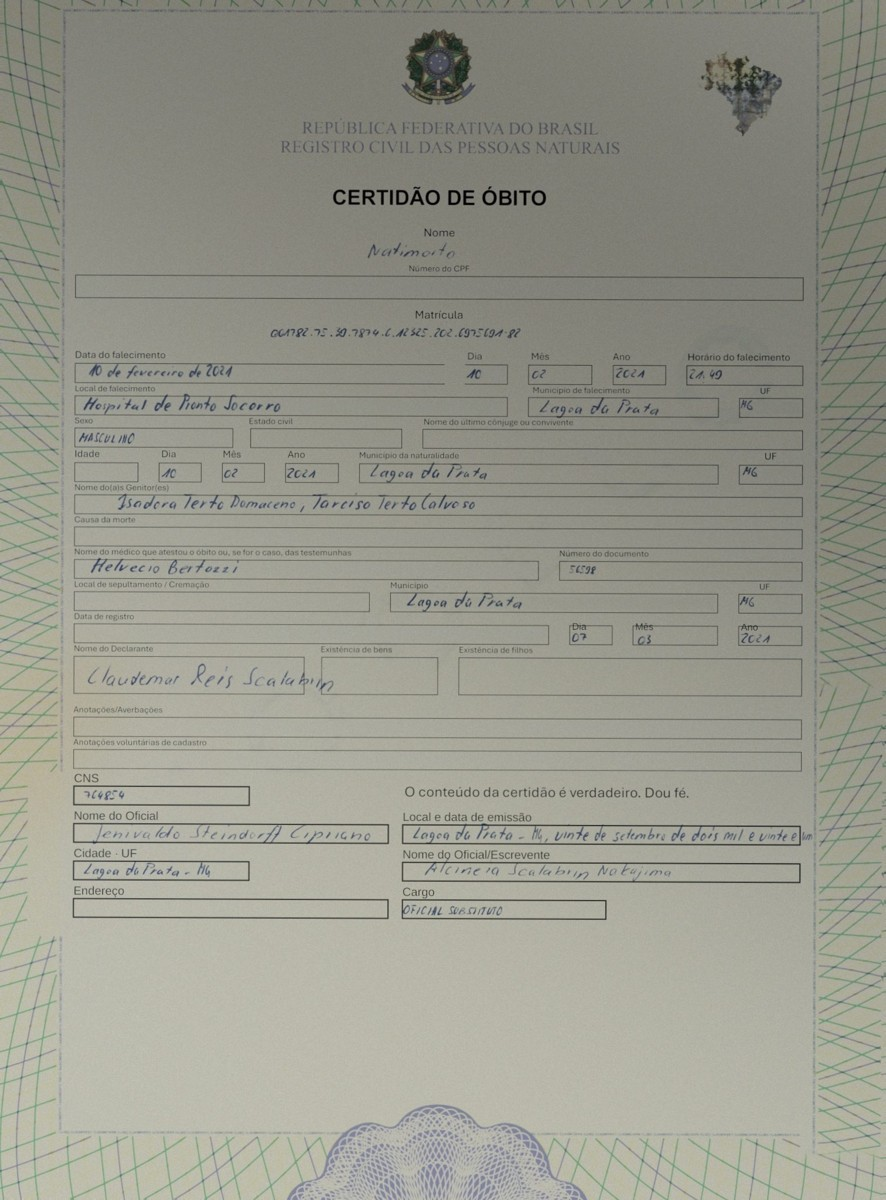
\includegraphics[height=63mm]{gerador_pagina.jpg}
\end{column}
\begin{column}{0.63\textwidth}
  \slidetitle{Gerador local de certidões}
  \vspace{3mm}
  \small
  \lbl{modelo} Modelos em branco e mapas de campos do OCRSD \thinrule
  \lbl{registro} Cada prenome, sobrenome e município é sorteado do léxico, respeitando a partição entre treino e teste \thinrule
  \lbl{escrita} Uma mão por página: 31 fontes manuscritas ou os geradores neurais VATr++ e Graves \thinrule
  \lbl{dificuldade} Quatro níveis, com letras deformadas, borrões, sombra, ruído e JPEG
\end{column}
\end{columns}
\end{frame}

\begin{frame}[plain]
\begin{tikzpicture}[remember picture,overlay]
  \node[inner sep=0] at (current page.center) {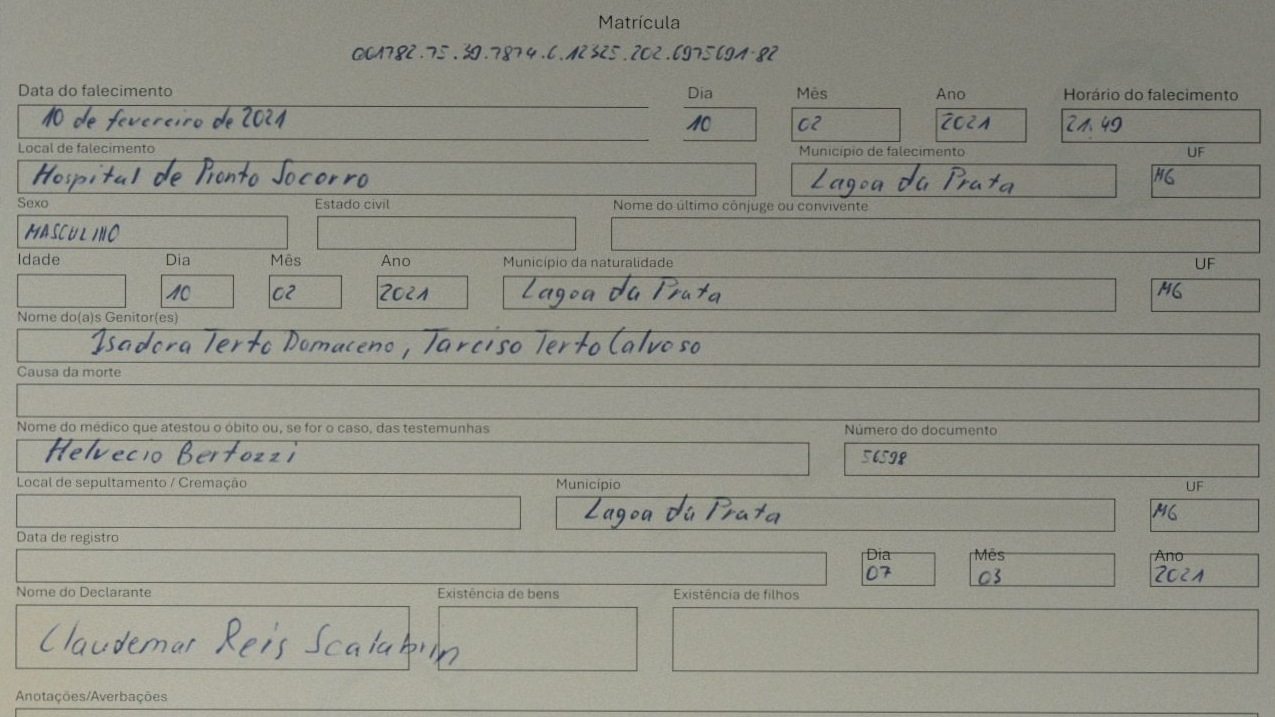
\includegraphics[width=\paperwidth]{gerador_cheia.jpg}};
\end{tikzpicture}
\end{frame}

% =====================================================================
% SEGURANÇA
% =====================================================================
\begin{frame}
\slidehead{Segurança}
\slidetitle{Segurança, privacidade e conformidade}
\vspace{4mm}
\small
\begin{columns}[t,onlytextwidth]
\begin{column}{0.30\textwidth}\coltop \lbl{ameaças}
  Extração de nomes do treino \thinrule
  Inferência de pertencimento \thinrule
  Injeção de instruções escritas na imagem \thinrule\end{column}
\begin{column}{0.30\textwidth}\coltop \lbl{riscos}
  Exposição de dados pessoais no treino \thinrule
  Nome errado aceito sem conferência \thinrule
  Uso do modelo fora do seu domínio \thinrule\end{column}
\begin{column}{0.30\textwidth}\coltop \lbl{controles}
  Nenhuma certidão real; nomes só como contagens \thinrule
  Nomes, fontes e escritores de teste fora do treino \thinrule
  Revisão humana das saídas marcadas \thinrule\end{column}
\end{columns}
\vfill
\sidenote{LGPD: minimização desde a coleta. Os testes de extração e de injeção ainda não foram executados.}
\vspace{2mm}
\end{frame}

% =====================================================================
% METODOLOGIA
% =====================================================================
\begin{frame}
\slidehead{Metodologia}
\slidetitle{Metodologia: de linhas para páginas}
\vspace{3.5mm}
\begin{columns}[T,onlytextwidth]
\begin{column}{0.53\textwidth}
  \coltop\lbl{etapa 1: linhas (lora\_v0)}
  \footnotesize
  \begin{tabular}{@{}lrr@{}}
  & Chandra & lora\_v0 \\
  \midrule
  CER no BRESSAY (\%) & 20,1 & \textbf{4,9} \\
  Nomes inéditos sem erro (\%) & 70,9 & \textbf{79,7} \\
  \midrule
  \multicolumn{3}{@{}l}{\textit{O mesmo adaptador em certidões inteiras}} \\
  Campos exatos, OCRSD (\%) & 84,7 & 84,4 \\
  Campos exatos, locais (\%) & 56,6 & 55,4 \\
  \end{tabular}
\end{column}
\begin{column}{0.42\textwidth}
  \coltop\lbl{etapa 2: páginas inteiras}
  \small
  \textbf{lora\_v1}: 1.800 páginas, a partir do Chandra \thinrule
  \textbf{lora\_v2}: mais 1.700 páginas, com peso maior nos nomes \thinrule
  Cerca de 65 min por etapa em uma RTX PRO 6000
\end{column}
\end{columns}
\vfill
\sidenote{O ganho em linhas não chegou às certidões, e por isso o treino passou para a página inteira.}
\vspace{2mm}
\end{frame}

% =====================================================================
% AVALIAÇÃO
% =====================================================================
\begin{frame}
\slidehead{Avaliação}
\slidetitle{Avaliação e critérios de sucesso}
\vspace{4mm}
\small
\begin{columns}[t,onlytextwidth]
\begin{column}{0.30\textwidth}\coltop \lbl{métricas}
  Acerto exato por campo, na região do campo \thinrule
  Nomes exatos \thinrule
  Truncamento, laço, memória e tempo \thinrule\end{column}
\begin{column}{0.30\textwidth}\coltop \lbl{cenários}
  Difícil: 100 páginas, 70\% das palavras de nome nunca vistas \thinrule
  Normal: 100 páginas, nomes pela frequência real \thinrule
  OCRSD, BRESSAY e XFUND-PT \thinrule\end{column}
\begin{column}{0.30\textwidth}\coltop \lbl{critérios de sucesso}
  Ganho com IC 95\% acima de zero (\emph{bootstrap} pareado) \thinrule
  Sem aumento de truncamento ou laço \thinrule
  Quantização com perda de até 1 ponto em nomes \thinrule\end{column}
\end{columns}
\end{frame}

% =====================================================================
% RESULTADOS
% =====================================================================
\begin{frame}
\slidehead{Resultados}
\slidetitle{Teste difícil: 55,4\% $\rightarrow$ 72,2\% dos campos}
\vspace{0.5mm}
\centering
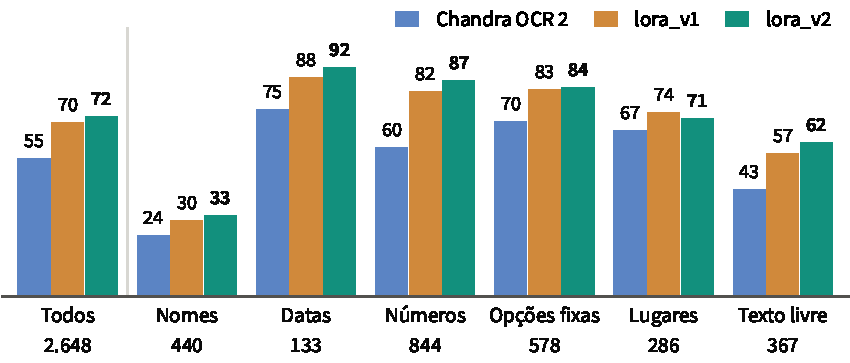
\includegraphics[width=\linewidth,height=61mm,keepaspectratio]{g_dificil.pdf}\par
\end{frame}

\begin{frame}
\slidehead{Resultados}
\slidetitle{Teste normal: 55,8\% $\rightarrow$ 72,0\% dos campos}
\vspace{0.5mm}
\centering
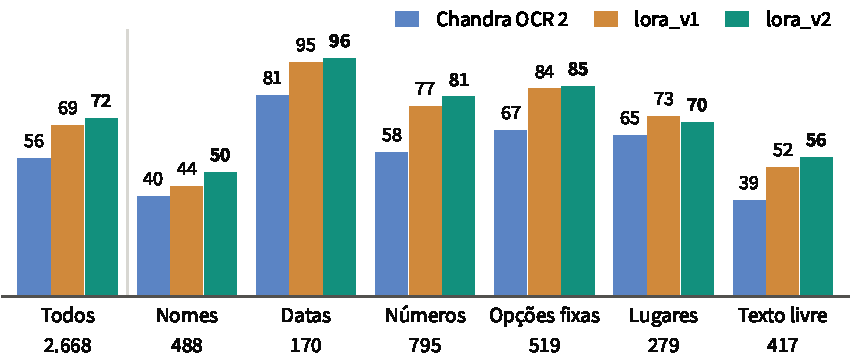
\includegraphics[width=\linewidth,height=61mm,keepaspectratio]{g_normal.pdf}\par
\end{frame}

\demonstracao{certidao_original.jpg}{Chandra OCR 2}{17}{errou matrícula, horário e nomes}
\demonstracao{certidao_ajustado.jpg}{lora\_v2}{20}{errou um prenome raro}

\begin{frame}
\slidehead{Resultados}
\slidetitle{Campos que o ajuste corrigiu}
\vspace{2mm}
\small
\setlength{\tabcolsep}{3pt}
\renewcommand{\arraystretch}{1.12}
\begin{tabular}{@{}m{6.1cm}m{3.95cm}m{3.95cm}@{}}
\toprule
Imagem & Chandra OCR 2 & lora\_v2 \\
\midrule
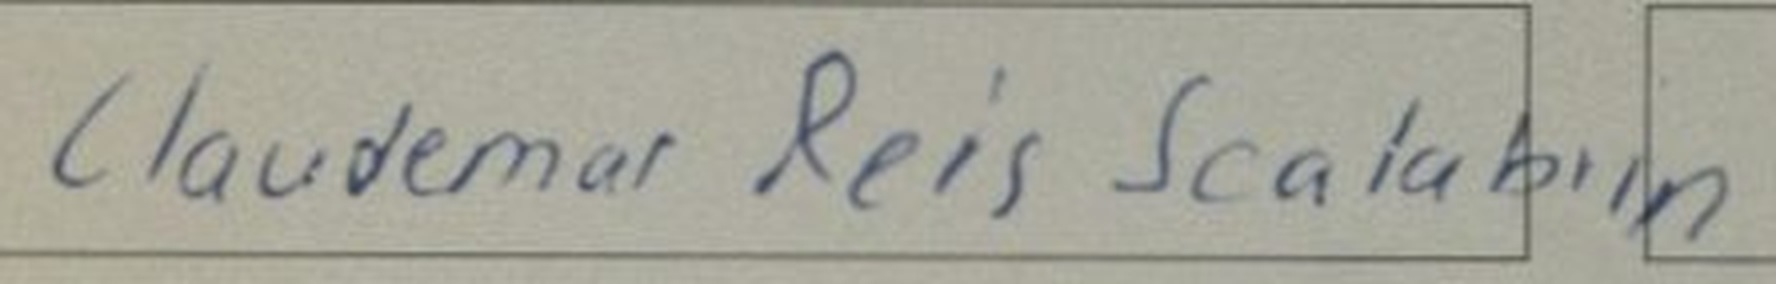
\includegraphics[width=5.95cm,height=11.5mm,keepaspectratio]{ex_claudemar.jpg} & Claude\erro{mi}r Reis Scalabrin & Claudemar Reis Scalabrin \\
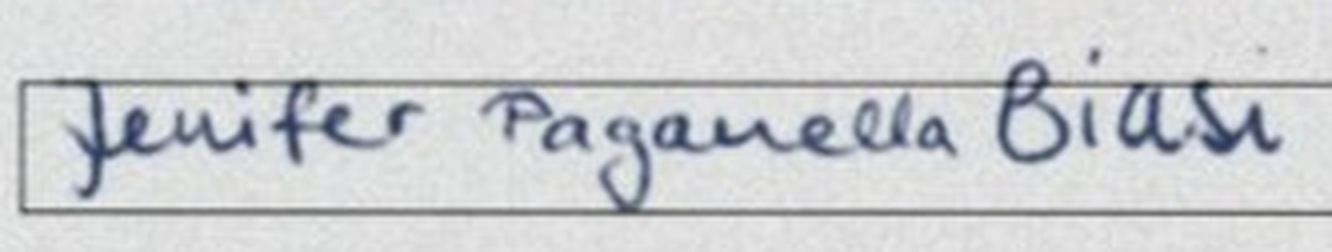
\includegraphics[width=5.95cm,height=11.5mm,keepaspectratio]{ex_jenifer.jpg} & Jenifer Paganella Bia\erro{ss}i & Jenifer Paganella Biasi \\
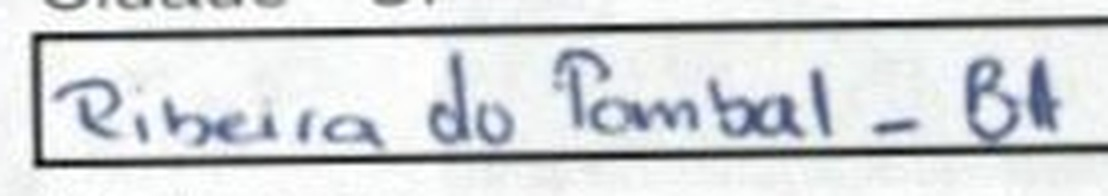
\includegraphics[width=5.95cm,height=11.5mm,keepaspectratio]{ex_ribeira.jpg} & Ribeira do \erro{T}ombal - BA & Ribeira do Pombal - BA \\
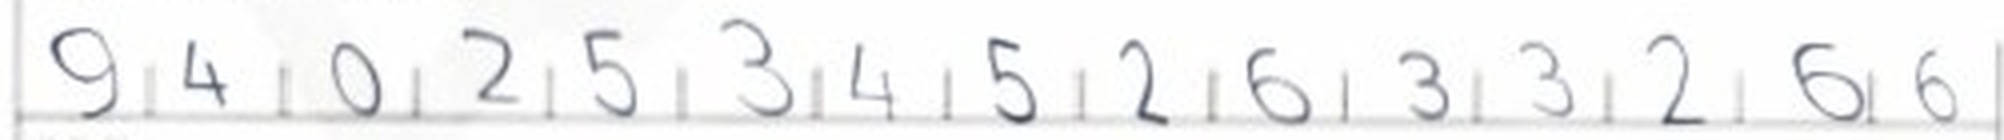
\includegraphics[width=5.95cm,height=11.5mm,keepaspectratio]{ex_sus.jpg} & 9\erro{1}0253452633266 & 940253452633266 \\
\bottomrule
\end{tabular}
\end{frame}

{
\setbeamertemplate{footline}{}
\begin{frame}
\slidehead{Resultados}
\slidetitle{Onde o modelo ainda erra}
\vspace{1.5mm}
\centering
\footnotesize
\setlength{\tabcolsep}{0pt}
\renewcommand{\arraystretch}{1.02}
\begin{tabular}{@{}p{4.8cm}p{4.8cm}p{4.8cm}@{}}
\toprule
\textcolor{tinta}{Gabarito} & \textcolor{tinta}{Chandra OCR 2} & \textcolor{tinta}{lora\_v2} \\
\midrule
\multicolumn{3}{@{}c@{}}{
\includegraphics[width=13.6cm,height=14mm,keepaspectratio]{ex_maikon.jpg}} \\
Maikon Giordano Cirino & \erro{Manoel} Giordan\erro{e} \erro{Critto} & \erro{Marcia} Giordan\erro{e} \erro{Critto} \\
\midrule
\multicolumn{3}{@{}c@{}}{
\includegraphics[width=13.6cm,height=14mm,keepaspectratio]{ex_guiomar.jpg}} \\
Guiomar Schiavon Arrabal & \erro{Geovana} Schiav\erro{e}n \erro{Ararabal} & \erro{Giovana} Schiav\erro{e}n \erro{Araral} \\
\midrule
\multicolumn{3}{@{}c@{}}{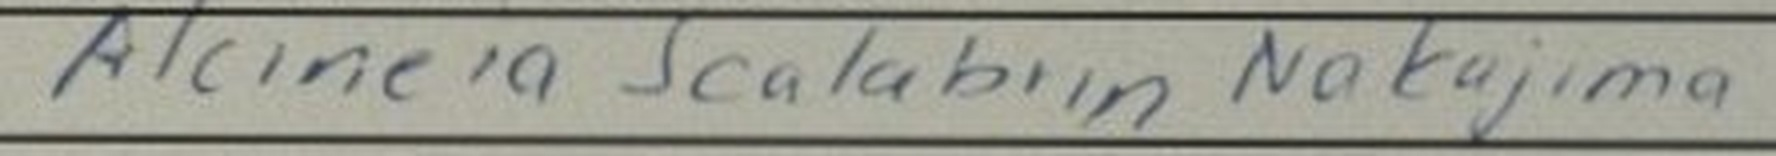
\includegraphics[width=13.6cm,height=14mm,keepaspectratio]{ex_alcineia.jpg}} \\
Alcineia Scalabrin Nakajima & Alcineia Scalabrin Nakajima & \erro{Alineia} Scalabrin Nakajima \\
\bottomrule
\end{tabular}
\end{frame}
}

\begin{frame}
\slidehead{Resultados}
\slidetitle{OCRSD: 84,6\% $\rightarrow$ 95,5\% dos campos}
\vspace{2.5mm}
\begin{columns}[T,onlytextwidth]
\begin{column}{0.58\textwidth}
  \footnotesize
  \renewcommand{\arraystretch}{1.1}
  \begin{tabular}{@{}lrrr@{}}
  \toprule
  Campos exatos (\%) & Campos & Chandra & lora\_v1 \\
  \midrule
  Todos & 1.460 & 84,6 & \textbf{95,5} \\
  Nomes & 399 & 84,7 & \textbf{95,5} \\
  Opções fixas & 244 & 74,6 & \textbf{98,8} \\
  Texto livre & 286 & 72,7 & \textbf{91,3} \\
  Lugares & 132 & 93,2 & \textbf{98,5} \\
  Datas & 94 & 98,9 & 98,9 \\
  Números & 305 & \textbf{95,4} & 94,4 \\
  \bottomrule
  \end{tabular}
\end{column}
\begin{column}{0.37\textwidth}
  \small
  \lbl{caligrafias fora do treino} {\rmfamily\Large 77,8\% $\rightarrow$ 94,0\%}\par\footnotesize 252 campos, escritores neurais reservados \thinrule
  \small
  \lbl{fontes também vistas no treino} {\rmfamily\Large 86,0\% $\rightarrow$ 95,8\%}\par\footnotesize 1.208 campos
\end{column}
\end{columns}
\vfill
\sidenote{94 páginas, avaliadas com o lora\_v1 antes de entrarem no treino do lora\_v2.}
\vspace{1.5mm}
\end{frame}

\begin{frame}[c,plain]
\centering
\normalsize
\renewcommand{\arraystretch}{1.17}
\setlength{\tabcolsep}{7pt}
\begin{tabular}{@{}lcc|c|ccc@{}}
\toprule
 & \multicolumn{2}{c|}{\textbf{Chandra OCR 2}} & \textbf{lora\_v1} & \multicolumn{3}{c}{\textbf{lora\_v2}} \\
 & BF16 & FP8 & BF16 & BF16 & FP8 & INT4 \\
\midrule
\multicolumn{7}{@{}l}{\textit{Teste difícil}} \\
\quad Campos exatos (\%) & 55,4 & 55,1 & 69,8 & \textbf{72,2} & 71,7 & 69,9 \\
\quad Nomes exatos (\%) & 24,3 & 24,3 & 30,5 & \textbf{32,5} & 30,7 & 28,9 \\
\multicolumn{7}{@{}l}{\textit{Teste normal}} \\
\quad Campos exatos (\%) & 55,8 & -- & 69,2 & \textbf{72,0} & 71,9 & 71,6 \\
\quad Nomes exatos (\%) & 40,4 & -- & 44,5 & \textbf{50,2} & 49,6 & 49,4 \\
\multicolumn{7}{@{}l}{\textit{Inferência (RTX PRO 6000, vLLM)}} \\
\quad Pesos na GPU (GiB) $\downarrow$ & 8,6 & 6,2 & 8,6 & 8,6 & 6,2 & \textbf{5,0} \\
\quad Uma página por vez (s) $\downarrow$ & 23,0 & -- & -- & 22,6 & 17,7 & \textbf{14,9} \\
\quad 48 por vez (s/página) $\downarrow$ & 1,25 & 1,20 & -- & 1,22 & 1,07 & \textbf{1,05} \\
\bottomrule
\end{tabular}
\end{frame}

\begin{frame}
\slidehead{Resultados}
\slidetitle{Fora das certidões, perde generalidade}
\vspace{2.5mm}
\begin{columns}[T,onlytextwidth]
\begin{column}{0.60\textwidth}
  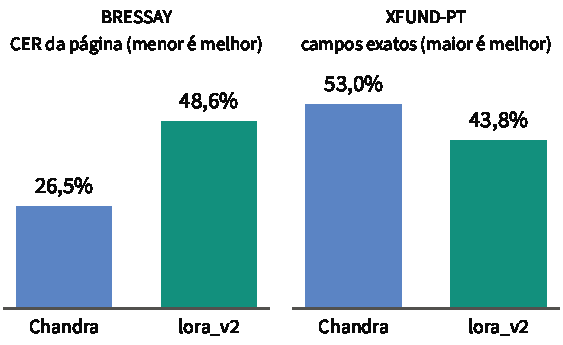
\includegraphics[width=\linewidth,height=56mm,keepaspectratio]{g_fora.pdf}
\end{column}
\begin{column}{0.36\textwidth}
  \small
  \lbl{principal limitação} O ajuste é específico para o Registro Civil; em outros tipos de documento, o Chandra original segue mais indicado \thinrule
  \lbl{bressay} 12 páginas do lora\_v2 e 13 do Chandra repetem texto até o limite. Nas outras 181, o CER vai de 6,8\% para 7,9\% \thinrule
  \lbl{xfund-pt} $-$9,2 pontos (IC $-$12,1 a $-$6,2)
\end{column}
\end{columns}
\end{frame}

% =====================================================================
% DISCUSSÃO
% =====================================================================
\begin{frame}
\slidehead{Discussão}
\slidetitle{Análise crítica}
\vspace{3mm}
\small
\begin{columns}[t,onlytextwidth]
\begin{column}{0.30\textwidth}\coltop \lbl{o que funcionou}
  Treinar na página inteira: nas mesmas 38 certidões, 56,6\% (Chandra), 55,4\% (linhas) e 73,2\% (páginas) \thinrule
  Nomes com palavra inédita: +18 pontos, contra +7 nos já vistos (teste normal)\end{column}
\begin{column}{0.30\textwidth}\coltop \lbl{limitações}
  Perda de generalidade fora das certidões \thinrule
  Nomes nunca vistos: 32,5\% exatos \thinrule
  Testes só sintéticos, nos mesmos 5 documentos do treino\end{column}
\begin{column}{0.30\textwidth}\coltop \lbl{trade-offs}
  INT4: 41\% menos memória, $-$3,6 pontos em nomes no teste difícil \thinrule
  Treino sintético atende à LGPD, mas especializa o modelo \thinrule
  Triagem por confiança: em linhas, um quarto dos erros passa sem marcação\end{column}
\end{columns}
\end{frame}

% =====================================================================
% PRÓXIMOS PASSOS
% =====================================================================
\begin{frame}
\slidehead{Encaminhamento}
\slidetitle{Próximos passos}
\vspace{4mm}
\small
\begin{columns}[t,onlytextwidth]
\begin{column}{0.30\textwidth}\coltop \lbl{curto prazo}
  Misturar outros documentos no treino \thinrule
  Testes de extração e de injeção\end{column}
\begin{column}{0.30\textwidth}\coltop \lbl{médio prazo}
  Validar com certidões reais, com autorização \thinrule
  Livros e certidões antigos\end{column}
\begin{column}{0.30\textwidth}\coltop \lbl{longo prazo}
  Ajuste contínuo com as correções dos operadores \thinrule
  Memória de correções\end{column}
\end{columns}
\end{frame}

% =====================================================================
% REFERÊNCIAS
% =====================================================================
\begin{frame}
\slidehead{Encaminhamento}
\slidetitle{Referências}
\vspace{3mm}
\fontsize{8.4}{10.6}\selectfont
\begin{columns}[T,onlytextwidth]
\begin{column}{0.48\textwidth}
  \coltop
  Datalab. Chandra OCR 2, 2026. \thinrule
  Hu et al. LoRA: Low-Rank Adaptation of Large Language Models. ICLR, 2022. \thinrule
  Neto et al. BRESSAY: A Brazilian Portuguese Dataset for Offline HTR, 2024. \thinrule
  Siqueira, T. OCRSD: Detecção, Redação e Síntese de Documentos de Registro Civil com IA, 2026. \thinrule
  Vanherle et al. VATr++. IEEE TPAMI, 2024. \thinrule
  Graves, A. Generating Sequences With Recurrent Neural Networks, 2013.
\end{column}
\begin{column}{0.48\textwidth}
  \coltop
  Xu et al. XFUND. Findings of ACL, 2022. \thinrule
  Kwon et al. Efficient Memory Management for LLM Serving with PagedAttention (vLLM). SOSP, 2023. \thinrule
  Carlini et al. Extracting Training Data from Large Language Models. USENIX Security, 2021. \thinrule
  IBGE. Estatísticas do Registro Civil 2023. \thinrule
  Brasil. Lei 13.709/2018 (LGPD).
\end{column}
\end{columns}
\end{frame}

% =====================================================================
% ENCERRAMENTO
% =====================================================================
\begin{darkframe}
\begin{frame}[plain]
\color{white}
\vspace{5mm}
\begin{columns}[T,onlytextwidth]
\begin{column}{0.72\textwidth}
  {\ttfamily\scriptsize\color{gold}ENCERRAMENTO}\hspace{2mm}%
  {\color{white!40!deepteal}\rule[1mm]{0.66\linewidth}{0.4pt}}\par
  \vspace{6mm}
  {\rmfamily\fontsize{21}{26}\selectfont De 56\% para 72\% dos campos manuscritos, sem treinar com dados de pessoas reais\par}
  \vspace{2.5mm}
  {\fontsize{12.5}{16}\selectfont O ajuste é específico para o Registro Civil; em outros tipos de documento, o Chandra original segue mais indicado. O próximo passo é validar com certidões reais.\par}
  \vspace{5mm}
  \hrulec{white!35!deepteal}{0.4pt}\vspace{2.5mm}
  {\small Obrigado!\par}\vspace{0.5mm}{\footnotesize\color{white!80}Agradeço ao tutor Lucas Mayr e ao Tiago Siqueira, pelo OCRSD\par}
  \vspace{1mm}
  {\ttfamily\footnotesize\color{white!85!deepteal}github.com/gabriel-salmoria/ai-sec}
\end{column}
\begin{column}{0.22\textwidth}
  \raggedleft
  \vspace{12mm}
  \colorbox{white}{\color{black}\qrcode[height=2.5cm]{https://github.com/gabriel-salmoria/ai-sec}}
\end{column}
\end{columns}
\end{frame}
\end{darkframe}

\end{document}
